% 35-26(35쪽) — 모든 실수에서 미분가능한 y=f(x)의 그래프와 x축 위의 네 점 a, b, c, d(각 점에서 그래프까지 세로 점선).
% 스캔 화질이 낮아 TikZ 로 다시 그림. 원문처럼 a 는 첫 봉우리의 증가 부분, b 는 둘째 봉우리의 꼭대기, c·d 는 셋째 봉우리의 증가·감소 부분에 둔다. 눈금·좌표값은 원문에 없다.
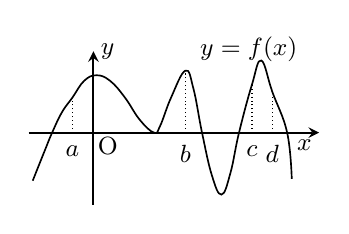
\begin{tikzpicture}[scale=0.235, line width=0.5pt]
  \draw[->, >=stealth, line width=0.7pt] (-3.5,0) -- (12.2,0) node[below left=-1pt, font=\small] {$x$};
  \draw[->, >=stealth, line width=0.7pt] (0,-3.9) -- (0,4.4) node[right=-1pt, font=\small] {$y$};
  \draw[line width=0.6pt] plot[smooth, tension=0.7] coordinates {
    (-3.28,-2.6) (-2.6,-0.9) (-2.23,0) (-1.7,1.1) (-1.13,1.9)
    (-0.5,2.8) (0.17,3.1) (0.9,2.8) (1.7,1.9) (2.5,0.7)
    (3.27,0) (3.6,0.35) (4.2,1.9) (4.97,3.35) (5.4,2.4)
    (5.87,0) (6.4,-2.3) (6.92,-3.35) (7.4,-2.2) (7.87,0)
    (8.57,2.6) (9.07,3.9) (9.67,2.2) (10.47,0) (10.72,-2.5)};
  \draw[densely dotted, line width=0.4pt] (-1.13,0) -- (-1.13,1.9);
  \draw[densely dotted, line width=0.4pt] (4.97,0) -- (4.97,3.35);
  \draw[densely dotted, line width=0.4pt] (8.57,0) -- (8.57,2.6);
  \draw[densely dotted, line width=0.4pt] (9.67,0) -- (9.67,2.2);
  \node[below=1pt, font=\small] at (-1.13,0) {$a$};
  \node[below=1pt, font=\small] at (4.97,0) {$b$};
  \node[below=1pt, font=\small] at (8.57,0) {$c$};
  \node[below=1pt, font=\small] at (9.67,0) {$d$};
  \node[below right=-2pt, font=\small] at (0,0) {$\mathrm{O}$};
  \node[font=\small] at (8.4,4.5) {$y=f(x)$};
\end{tikzpicture}
